\documentclass{acm_proc_article-sp}
\bibliographystyle{unsrt}

\begin{document}

\title{A Web-Based Editor for Multiplayer Choice Games}
\numberofauthors{1}
\author{
% 1st. author
\alignauthor
Ian Holmes\\
       \affaddr{Department of Bioengineering}\\
       \affaddr{University of California}\\
       \affaddr{California, Berkeley}\\
       \email{ihh@berkeley.edu}
}
\date{30 November, 2013}

\maketitle
\begin{abstract}
The structure of a choice-driven interactive story can be modeled as a syntax tree, generated by a player
 from a grammar, which in turn was generated by a game author.
Using this grammar metaphor, ``Boswell'',
 a web-based Integrated Development Environment,
 was developed for writing, testing, playing and sharing choice-based interactive fiction scripts.
The system includes a domain-specific language,
 a map overview, a parse-tree debugger, and a network client for multiplayer games.
\end{abstract}

% A category with the (minimum) three required fields
%\category{H.4}{Information Systems Applications}{Miscellaneous}
%A category including the fourth, optional field follows...
%\category{D.2.8}{Software Engineering}{Metrics}[complexity measures, performance measures]


\section{Introduction}

Choice-based interactive fiction came of age in the 1980's:
Choose Your Own Adventure\cite{packard1982cave}, Fighting Fantasy\cite{jackson1982warlock},
and Lone Wolf are well-known imprints.
The genre has seen an early 21st-century resurgence with the advent of writing
tools---from domain-specific languages like ChoiceScript\cite{ChoiceScript},
to interactive editors like Twine\cite{Twine} and Inklewriter\cite{Inklewriter}---which
have lowered the barriers to game creation and increased the diversity of authorial voices.

A simple choice-based story can be compared to a flowchart, or a state machine,
or (in the language of grammar theory) a {\em regular grammar}.
The main control-flow construct is the optional {\tt GOTO} statement
(``{\em IF you choose to take the chalice, TURN TO page 400}'').
The structure of the story is a linear progression of scenes:
 the game program is a finite state machine that outputs scenes in a player-driven sequence.

In modeling many kinds of text, it is often useful to allow a richer structure.
For example, conversations often make diversions (sometimes nested diversions (and sometimes multiply nested))
before returning to the main theme.
Epic adventures can include side-quests; stories often have epilogues.

This sort of structure can be modeled using a {\em context-free grammar} (CFG).
If a typical choice-based story (with a regular grammar) is akin to a state machine,
 whose main control-flow construct is {\tt GOTO},
then a CFG-based story is like a pushdown automaton (a finite-state machine with a stack)
 which allows not only {\tt GOTO} but also {\tt GOSUB}.

In this abstract we describe Boswell, a software system that allows authoring of story CFGs
via an interface inspired by graphical editors like Twine and domain-specific languages like ChoiceScript.
The created games can be played over the web by multiple players in different locations.

To extend choice-based stories in this way might indicate an excessive fondness for formalism.
However, a well-defined framework provides a robust foundation, as well as a rich variety of links to other areas of culture.
Grammars have variously served as metaphysical systems\cite{Ashtadhyayi,luhtala2005grammar},
tools of social unification and control\cite{AcademieFrancaise,RobertLowth},
and models of natural language\cite{Durbin98}.
They have been used in compiler theory\cite{aho2007compilers},
DNA sequence analysis\cite{Durbin98}, and
computer graphics\cite{LSystems}.
There is a literature on game-theoretic analysis of grammar-based games
\cite{DBLP:conf/icalp/EtessamiWY08}.
Templates and scripts for social interactions
 have a rich history in popular social psychology\cite{berne1973games,berne1973you}.
All of the above influences offer a source of inspiration for single- and multiplayer game design.

\section{Design}

\subsection{Game language}

The application is based around
a declarative, domain-specific language for specifying an attributed CFG.

The core element in this grammar, syntactically and semantically, is the {\em transformation rule},
delineated by curly braces and the two characters ``{\tt =>}''
\begin{verbatim}
 @scene
  => { This is a hint.
   => This is its expansion, leading to @next_scene. }
\end{verbatim}
In this, ``{\tt @scene}'' and ``{\tt @next\_scene}'' are labels denoting (respectively) the current and upcoming scenes;
``{\tt This is a hint}'' is {\em hint text} presented to the player as a choice;
and ``{\tt This is its expansion, leading to @next\_scene}'' is the {\em expansion text} generated if the player makes this choice
(note that the expansion text includes another scene label).

A block of transformation rules represents a list of choices:
\begin{verbatim}
 @scene => { First hint => First expansion
           | Second hint => Second expansion
           | Third hint => You get the picture }
\end{verbatim}
Any number of ``{\tt hint => expansion}'' rules are allowed.
Rules can also be declared separately:
\begin{verbatim}
 @scene => { First hint => First expansion }
 @scene => { Second hint => Second expansion }
 @scene => { Third hint => You get the picture }
\end{verbatim}

An optional longer form includes additional text fields:
\begin{verbatim}
 @scene => [ Preamble | Placeholder | Prompt ]
           { Hint 1 => Expansion 1
           | Hint 2 => Expansion 2
           | Hint 3 => Expansion 3 ... }
\end{verbatim}

Here, {\tt Preamble} is text describing the scene;
{\tt Placeholder} is text temporarily displayed at the bottom of the scene (before the list of choices),
and deleted when an expansion is selected;
and {\tt Prompt} is text, also transiently displayed, that is associated with the list of choices.

Typically the prompt takes the form of a question addressed directly to the player:
\begin{verbatim}
 @unrest =>
[ "Sire, the peasants are revolting."
  | _So tedious..._ 
  | What will you do? ] 
{ Feed them.
   => You cast grain from the battlements.
      @peace
| Play some music.
   => No lute can drown their hungry groans.
      @revolt }
\end{verbatim}

The preamble ``{\em So tedious...}'' will disappear when a selection is made; being wrapped in underscores, the words will also appear in italics, as a result of the Markdown-like macro transformation.
The prompt ``What will you do?'' will also disappear when a selection made.
(In multiplayer mode, the prompt is only shown to the active player.)

An expansion can contain multiple scene labels, or none. This feature distinguishes the CFG from the less-expressive regular grammar.
From the viewpoint of automata theory, it implies a pushdown stack, a.k.a. {\tt GOSUB}.
This is good for scheduling scenes in sequence, e.g. the four stages of the Hero's Journey
\begin{verbatim}
 @quest =>
 [ Do you accept the Monomyth?? ]
 { No => Have a happy life eating mush.
 | Yes => @separate @descend @ascend @unify }
\end{verbatim}


In the terminology of formal grammar theory: the scene labels ({\tt @scene}, {\tt @quest}, {\tt @next\_scene}) which appear before the first ``{\tt =>}'' sign and also (sometimes) flanked by text in the expansions, are {\em nonterminal symbols}.
Each expansion is a mixture of {\em terminal symbols} (ordinary rendered text, consisting of HTML tags and ASCII characters) and nonterminal symbols.

Nonterminal symbols denote points in the text (scenes) where further expansion is possible;
terminal symbols denote static endpoints of the text.
The preamble, placeholder, prompt and hint are {\em attributes}
added to make the grammar formalism a little more friendly to writing interactive stories.

All nonterminal symbols begin with {\tt @}.
Special characters such as {\tt \$@[]\{\}} can be escaped with a backslash if required in the text.
Quotation marks and other common punctuation are not special characters and can be used directly, as can HTML tags.
Some syntactic sugar for HTML tags (e.g. flanking underscores for italics) is borrowed from Markdown \cite{Markdown}.

Starting from a designated initial nonterminal (named {\tt @start} by default),
iterated application of these rules generates a {\em parse tree} (Figure~\ref{fig:tree}, right),
with nonterminal symbols at internal nodes and terminal symbols at the tips.
The final text can be read off from the terminals at the leaf nodes (Figure~\ref{fig:tree}, left).

\begin{figure}
\fbox{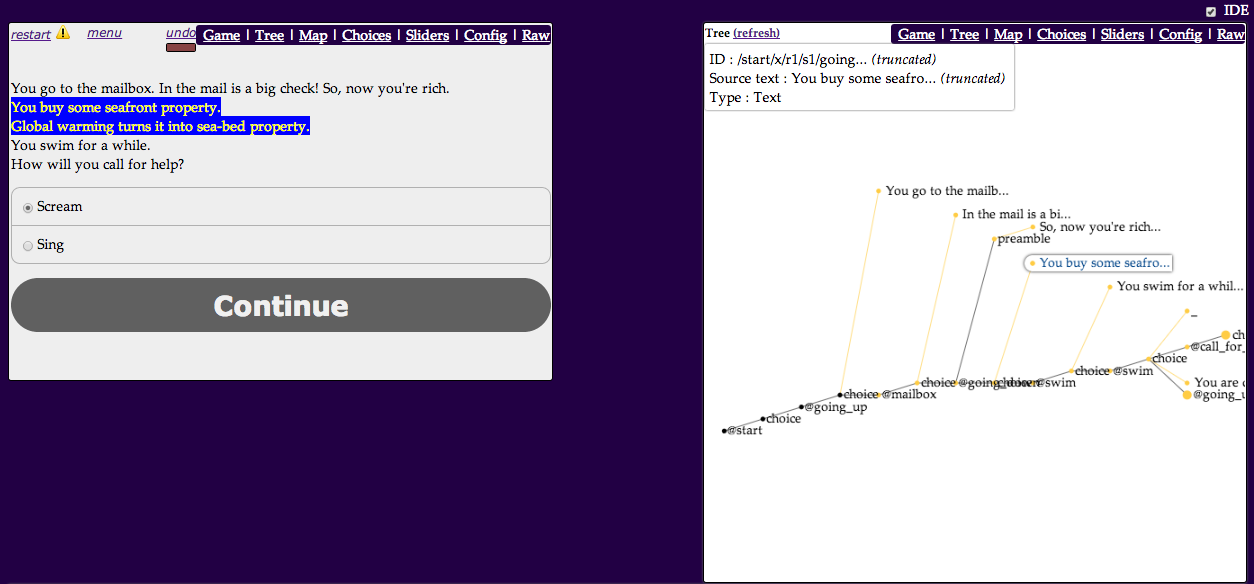
\includegraphics[width=\columnwidth]{ParseTree.png}}
\caption{
\label{fig:tree}
The parse tree visualization (right) helps debug gameplay (left).
}
\end{figure}

The sequence of terminals is post-processed before being rendered,
so the terminals themselves do not necessarily correspond exactly to what is shown on screen.
Specifically, the terminal nodes at the leaves of the parse tree represent a {\em program text},
which can contain embedded commands (such as variable assignments, inputs, modification, and interpolation)
that are then interpreted to (deterministically) compute the {\em story text} presented to the player.
As noted above, a Markdown-like macro expansion is further applied to the generated story text,
for quick HTML styling \cite{Markdown}.

Extra keywords are available; for example, to specify that some variables are directly controlled by the player,
(using sliders), or to delineate a variable as the score.
Other keywords can specify the game title, or control the behavior of the ``undo'' button.

Not all transformation rules need be presented to the player at every opportunity.
The author can flag individual rules to be hidden from view some fixed number of times
before first being shown, or limited to some finite number of uses.
Various modifier keywords can be associated with nonterminals to indicate this in the game source file.

More computationally expressive logic for controlling story flow is available via the use of computer players.
For nonterminals that are flagged as belonging to the computer player,
rules are normally played at random,
but this behavior can be manipulated by the author to
assign different probabilistic weights to the rules
(and these weights can also be boolean logic expressions, allowing for more sophisticated control of flow).
The player can also ``steer'' the computer player by manipulating probabilistic weight parameters directly,
by means of slider controls in the HTML page.

\subsection{Editor}

\begin{figure}
\fbox{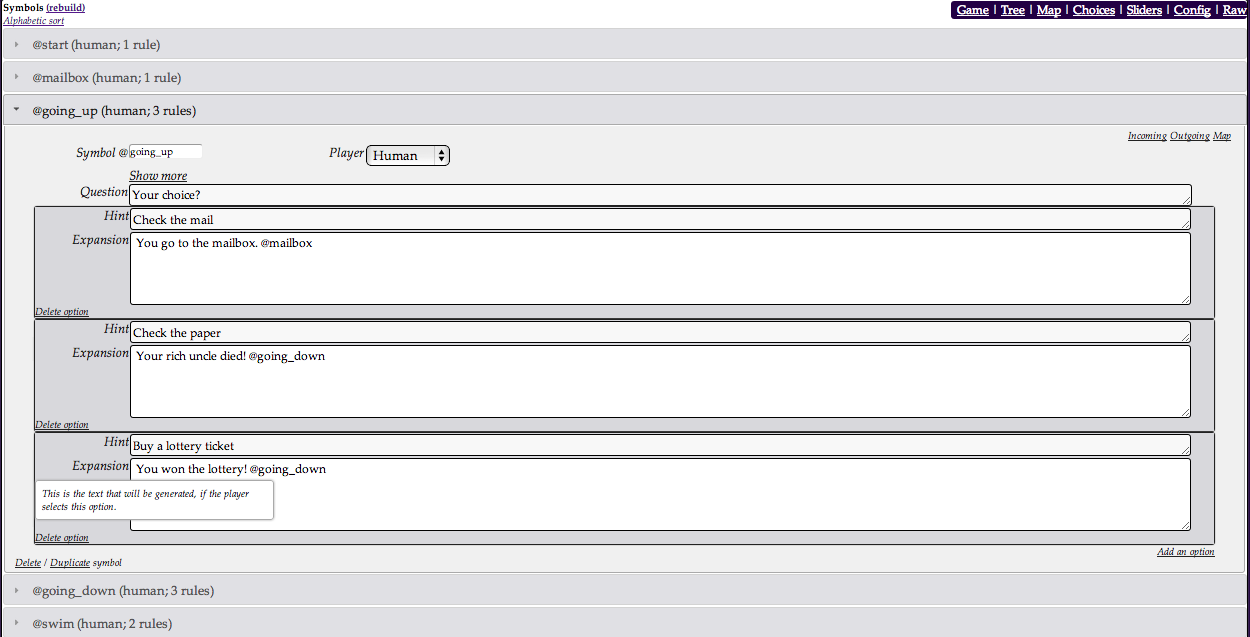
\includegraphics[width=\columnwidth]{Editor.png}}
\caption{
\label{fig:editor}
The nonterminal pane allows drag-and-drop ordering and editing of menus.
}
\end{figure}

At the most basic level, the editor includes a textbox for direct editing of game source code.
Beyond this, a number of User Interface (UI)
elements are presented together as a basic Integrated Development Environment (IDE).

The main element is a drag-and-drop sortable list of nonterminal editing panes (Figure~\ref{fig:editor}).
Each nonterminal pane contains a drag-and-drop-sortable list of transformation rules,
together with UI elements for modifying rule behavior (e.g. the number of times
a rule can be used by, or should be hidden from, the player).
An overview summarizes orphan nonterminals (never generated by any rules),
bare nonterminals (no text), and empty rules (loose ends).
Hyperlinks are provided for quick navigation to incoming/outgoing nonterminals,
and also to the map view.

Another drag-and-drop sortable list specifies the parameters that the player
can set directly via slider controls.
Some properties of the grammar (e.g. its title) can be directly edited.

\subsection{Map}

\begin{figure}
\fbox{
\includegraphics[width=\columnwidth]{Map.png}}
\caption{
\label{fig:map}
The map provides an overview of connections between nonterminals.
}
\end{figure}

The map, rendered using a third-party graph visualization library,
shows the overall structure of the game (Figure~\ref{fig:map}).
Nodes represent nonterminals (arranged in a circular layout).
Edges $a \to b$ imply the existence of at least one rule $a \to \ldots b \ldots$
with $a$ on the left-hand side and $b$ on the right.

Nodes are colored to represent some useful information
(e.g. whether the corresponding nonterminal is human- or player-controlled,
whether it is a loose end, and so forth).
The author can mouse-over a node to highlight incoming \& outgoing edges.

\subsection{Parse tree debugger}

The parse tree is visualized using the same graph library as the map (Figure~\ref{fig:tree}, right).
The various types and status of nodes (terminals; expanded \& unexpanded nonterminals (player- and computer-controlled); parameter references, assignments \& inputs) is indicated via size and coloring.
The tester can mouseover nodes to highlight the expanded text, and see order and time of expansion.
Clicking on a node navigates to the corresponding nonterminal pane in the editor.

\subsection{Game client}

The parse tree is rendered as text after performing variable substitutions (Figure~\ref{fig:tree}, left).
Minimal styling is used to present choice lists and animate key events,
e.g. fading-in of newly-rendered text.

An ``undo'' button with gradually-increasing recharge time is offered as an optional game mechanic for solo play.
(The complications of implementing multiplayer ``undo'' were eschewed.)

\subsection{Multiplayer operation}

Multiplayer mode is enabled by increasing the number of {\em roles} in the grammar from its default value of 1.
The number of roles is the same as the number of (human) players.
Each nonterminal node in the parse tree is controlled (i.e. can only be expanded) by the player in one specific role.
This prevents race conditions by design: each choice is uniquely controlled by one player.
The {\tt @start} nonterminal at the root node is always controlled by the player in the first role.
By default, if node $X$ is controlled by role $n$ and there are $k$ roles,
then all children of node $X$ are controlled by role $((n+1)\mod k)$.
Thus, control passes predictably from one player to the next,
although this default behavior can be modified by the author (e.g. to indicate that a particular nonterminal
should always be controlled by a given role).
For every role, there is one human player (for manual choices)
and one computer player (for automatic choices).

Multiplayer mode is implemented using a third-party publish-subscribe (pub-sub) framework.
Games are organized on an invitation channel and then take place on an hierarchically-structured
set of play channels, with one channel for each node of the parse tree.
CSS animations report
 (a) publication of rules to the pub-sub server (for locally-controlled node expansions),
 (b) subscription of a listener at a particular point in the parse tree (for remotely-controlled nodes).

\section{Discussion}

Grammars are found throughout computer science,
and there are many potential applications of an
integrated system for designing grammars and then using them collaboratively to generate texts over a network.
Such applications range from
serious uses in IT enterprise (e.g. structured chat-rooms for product support),
through traditional game tropes (e.g. dungeonmaster-player conversations),
through new electronic models of social interaction (e.g. scripted interactive dates).

% Below, we discuss some possible extensions.

\subsection{Cryptographic signatures}

Cryptographically-authenticated play would obviate the need for a server or central scoring authority.
A cryptographic extension of the basic pub-sub model should be straightforward.
Crucial messages must be signed (and counter-signed when received):
these include invitations, applications to join the game, and rule expansions.

\subsection{Strategic optimality}

Strategically optimal algorithms for playing this kind of game are known to exist when the scoring scheme is a trivial function of the parse tree (e.g. fixed rewards for using certain nonterminals \cite{DBLP:conf/icalp/EtessamiWY08}).
However, the scoring scheme described here is considerably more flexible, modeling many aspects of context-sensitive grammars as well as CFGs.

The programming language for the computer player does not attempt to model AI in any deep sense:
it is very simple, just offering variables, conditional tests, and the in-built facility for looping and recursion that comes for free with the CFG.

A possible extension is to use an ambiguous grammar (multiple parse trees consistent with observed output)
and introduce a computer player that can parse the current output
(e.g. using Earley-Stolcke parsing \cite{Stolcke:1995:EPC:211190.211197})
and predict future outcomes probabilistically.

\section{Implementation}

Implemented in JavaScript
using SigmaJS, PegJS, JQuery, OpenPGP, Node, and Faye,
with CSS from ChoiceScript.
Tested in Google Chrome and Mozilla Firefox.

% An early choice-based engine prototype ({\em Schooz}) was developed in Scheme.
% A prototype parser-driven AI ({\em Gertie}) was developed in Perl.


\subsection{Availability}

Code is freely available at
{\tt https://github.com/ihh/banterscribe}


\subsection{Acknowledgements}

Many thanks are due Dan Fabulich, Richard Evans, Michael Mateas, Noah Wardrip-Fruin,
Emily Short, Graham Nelson, Jon Ingold,
and Rudy Rucker for help and inspiration.


\bibliography{lwpaper}

\balancecolumns
% That's all folks!
\end{document}
